Il guadagno intrinseco ($A_{vi}$) è definito come il massimo guadagno ottenibile da un MOSFET, polarizzato da un generatore di corrente ideale. Fornisce una misura di quanto un MOSFET può amplificare senza essere influenzato da elementi esterni. Esso viene calcolato come:

$$A_{vi} = g_{m} \cdot r_0 = \frac{g_{m}}{g_{ds}} $$

Con $g_m$ la transconduttanza e $r_0$ la resistenza in uscita dal transistor (${1}/{g_{ds}}$). Spesso, il grafico di $A_{vi}$, viene mostrato in funzione del coefficiente di inversione ($I_{C0}$), parametro utile per descrivere il grado di inversione del canale (debole: per valori inferiori a $0.1$, moderata: tra $0.1$ e $10$, forte: superiori a $10$) il quale si può ricavare dalla $I_d$ ad alte $V_{ds}$:

$$I_{C0} = \frac{I_{d}}{I_{z}^{*}} \cdot \frac{L}{W}$$

La corrente caratteristica ($I_{z}^{*}$) è stata misurata pre-irraggiamento. I valori sono riportati nella tabella \ref{tab:corrente_caratteristica}.

\begin{table}[ht]
    \centering
    \begin{tabular}{c c}
        \toprule
        Tipologia Canale & $I_{z}^{*}$ \\
        \midrule
        N                & $470nA$     \\
        P                & $370nA$     \\
        \bottomrule
    \end{tabular}
    \caption{Valori della corrente caratteristica misurati prima dell'irraggiamento}
    \label{tab:corrente_caratteristica}
\end{table}


Nelle figure \ref{fig:guadagnoIntrinseco_N} e \ref{fig:guadagnoIntrinseco_P} (NMOS e PMOS) vengono mostrati i grafici $A_{vi}$ - $I_{C0}$, raggruppati per larghezza di canale, prima e dopo l'irraggiamento a $3Grad$.

Mentre nei NMOS si nota un innalzamento significativo della curva $A_{vi}$ - $I_{C0}$, soprattutto per lunghezze di canale più grandi. Questo non sembra verificarsi per i PMOS, infatti, l'offset della curva è leggermente negativo rispetto ai rispettivi grafici pre-irraggiamento. Effetto più visibile per le lunghezze di canale più grandi.
\todo[inline]{Dare una spiegazione a questo effetto(?), e magari riscriverla meglio}  


\begin{figure}[ht]
    \centering
    %W = 100
    \includegraphics[width=0.49\textwidth]{./capitolo2/Guadagno_Intrinseco/NMOS/pre/Guadagno_Intrinseco_W-100}
    \includegraphics[width=0.49\textwidth]{./capitolo2/Guadagno_Intrinseco/NMOS/3Grad/Guadagno_Intrinseco_W-100}
    %W = 200
    \includegraphics[width=0.49\textwidth]{./capitolo2/Guadagno_Intrinseco/NMOS/pre/Guadagno_Intrinseco_W-200}
    \includegraphics[width=0.49\textwidth]{./capitolo2/Guadagno_Intrinseco/NMOS/3Grad/Guadagno_Intrinseco_W-200}
    %W = 600
    \includegraphics[width=0.49\textwidth]{./capitolo2/Guadagno_Intrinseco/NMOS/pre/Guadagno_Intrinseco_W-600}
    \includegraphics[width=0.49\textwidth]{./capitolo2/Guadagno_Intrinseco/NMOS/3Grad/Guadagno_Intrinseco_W-600}

    \caption{Variazioni del guadagno intrinseco per un NMOS, a sinistra pre-irraggiamento mentre a destra dopo una dose di $3Grad$}
    \label{fig:guadagnoIntrinseco_N}
\end{figure}


\begin{figure}[ht]
    \centering
    %W = 100
    \includegraphics[width=0.49\textwidth]{./capitolo2/Guadagno_Intrinseco/PMOS/pre/Guadagno_Intrinseco_W-100}
    \includegraphics[width=0.49\textwidth]{./capitolo2/Guadagno_Intrinseco/PMOS/3Grad/Guadagno_Intrinseco_W-100}
    %W = 200
    \includegraphics[width=0.49\textwidth]{./capitolo2/Guadagno_Intrinseco/PMOS/pre/Guadagno_Intrinseco_W-200}
    \includegraphics[width=0.49\textwidth]{./capitolo2/Guadagno_Intrinseco/PMOS/3Grad/Guadagno_Intrinseco_W-200}
    %W = 600
    \includegraphics[width=0.49\textwidth]{./capitolo2/Guadagno_Intrinseco/PMOS/pre/Guadagno_Intrinseco_W-600}
    \includegraphics[width=0.49\textwidth]{./capitolo2/Guadagno_Intrinseco/PMOS/3Grad/Guadagno_Intrinseco_W-600}

    \caption{Variazioni del guadagno intrinseco per un PMOS, a sinistra pre-irraggiamento mentre a destra dopo una dose di $3Grad$}
    \label{fig:guadagnoIntrinseco_P}
\end{figure}